\documentclass{article}[18pt]
\usepackage[utf8]{inputenc}
\usepackage[margin=0.7in]{geometry}
\usepackage{amsmath}
\usepackage{titlesec}
\usepackage{pgfplots}
\usepackage{graphicx}
\usepackage[english]{babel}
\usepackage{fancyhdr}
\usepackage{gensymb}
\usepackage{tabularx}
\usetikzlibrary{decorations, decorations.text,positioning,quotes,arrows.meta,decorations.markings,3d,shapes,decorations.pathmorphing}
\pgfplotsset{width=10cm,compat=1.9}
\usepackage[super]{nth}
\titlespacing\section{0pt}{14pt plus 4pt minus 2pt}{0pt plus 2pt minus 2pt}
\newlength\tindent
\setlength{\tindent}{\parindent}
\setlength{\parindent}{0pt}
\renewcommand{\indent}{\hspace*{\tindent}}
\hyphenpenalty =10000
\pagestyle{fancy}
\fancyhf{}
\rhead{Sam Robbins 13SE}
\lhead{A Level Physics - Nuclear Physics}
\rfoot{Page \thepage}
\usepackage{mathtools}
\usetikzlibrary{calc,quotes,angles}
\tikzstyle{arrow} = [thick,->,>=stealth]
\begin{document}
\begin{center}
\underline{\huge Nuclear energy}
\end{center}
\section{Energy and mass}
\subsection{Annihilation and Pair production}
When a particle and its corresponding particle meet, they \textbf{annihilate} each other, and two gamma photons are produced, each with energy $mc^2$ where m is the mass of the particle.\\
\\
A single gamma photon of energy in excess of $2mc^2$ can produce a particle and an antiparticle, each of mass m, in a process called \textbf{pair production}.
\subsection{Energy changes in reactions}
$$\textrm{Energy released:} \ Q=\Delta mc^2$$ 
In any change where energy is released, such as radioactive decay, \textbf{total mass after $<$ total mass before} as some of the mass has been turned into energy, which has been released.
\begin{itemize}
\item In \textbf{Alpha Decay} the nucleus recoils when the $\alpha$ particle is emitted so the energy released is shared between the $\alpha$ particle and the nucleus. Conservation of momentum shows the energy released is shared between the $\alpha$ particle and the nucleus in inverse proportion to their masses.
\item In \textbf{Beta Decay} the energy released is shared between the $\beta$ particle, the nucleus and the neutrino/antineutrino. The vast majority of the energy goes with the $\beta$ particle and some of it with the nucleus.
\item In \textbf{Electron Capture} the nucleus emits a neutrino which carries away the energy released in the decay. The atom also emits an X-Ray photon when the inner shell vacancy is filled.
\end{itemize}
\subsubsection{Example Calculation}
\textit{The polonium isotope $^{210}_{84}Po$ emits $\alpha$ particles and decays to form the stable isotope of lead $^{206}_{82}Pb$. Write down an equation to represent this process and calculate the energy released when a $^{210}_{84}Po$ nucleus emits an $\alpha$ particle.\\
Mass of a $^{210}_{84}Po$ Nucleus=$209.93667u$\\
Mass of a $^{206}_{82}Pb$ Nucleus=$205.92936u$\\
Mass of a $\alpha$ particle=$4.00150u$\\
$1u=931.3MeV$}\\
$$^{206}_{82}Pb\rightarrow \ ^4_2\alpha+^{206}_{82}Pb+\textrm{Energy released}$$
$$\textrm{Mass difference}=\textrm{Total initial mass-total final mass}$$
$$\textrm{Mass difference}=209.93667-(205.92936+4.00150)$$
$$\textrm{Mass difference}=5.81\times10^{-3}u$$
$$\textrm{Energy released:}\ Q=\textrm{Mass difference in u}\times931.3=5.41MeV$$
\subsection{The strong nuclear force}
\begin{itemize}
\item The strength of the strong nuclear force can be estimated by working out the force of repulsion between two protons at a separation of 1fm(The approximate size of the nucleus). The strong nuclear force must be about the same magnitude as this force. This gives a value around 200N
\item The range of the strong nuclear force is no more than around 3-4fm. Experiments to measure the size of a nucleus show that nucleons are evenly spaced around 1fm apart, meaning that the strong force only acts between neighbour nucleons.
\item The energy needed to pull a nucleon out of the nucleus is on the order of MeV. This can be found from the force and distance to find the work done. $200\times3.5\times10^{-15}=4MeV$
\item The strong nuclear force must become repulsive at less than 0.5fm, otherwise the nucleus would compress further.
\end{itemize}
\newpage
\section{Binding energy}
\begin{center}
The \textbf{binding energy} of the nucleus is the work that must be done to separate a nucleus into its constituent neutrons and protons.
\end{center}
\begin{center}
The \textbf{mass defect}($\Delta m$) of a nucleus is defined as the difference between the mass of the separated nucleons and the mass of the nucleus. This exists as work is done to make a nucleus, reducing mass
\end{center}
\subsubsection{Mass defect calculation}
Nucleus of an isotope $^A_ZX$ has:\\
Z Protons\\
A-Z Neutrons\\
Mass=$M_{NUC}$
$$\textrm{Mass defect:} \ \Delta m=Zm_p+(A-Z)m_n-M_{NUC}$$
Where:\\
$m_p=\textrm{Mass of proton} \quad m_n=\textrm{Mass of neutron}$
\subsubsection{Binding energy calculation}
$$\textrm{Binding energy of a nucleus}=\Delta mc^2$$
When calculating with multiply the Mass defect in u by the MeV equivalent of 1u (931.3)
\subsection{Alpha particle tunnelling}
In a sufficiently large nucleus two protons and two neutrons may join together as a cluster. Because an alpha particle has a high binding energy the alpha particle gains enough energy to have a possibility of quantum tunnelling through the nucleus
\subsection{Nuclear stability}
The binding energy of each nuclide is different. The \textbf{binding energy per nucleon} of a nucleus is the average work done per nucleon to remove all the \textbf{nucleons} from a nucleus and so is a measure of the stability of a nucleus.\\
\\
If the binding energies per nucleon of two different nuclides are compared, the nucleus with more binding energy per nucleon is the more stable of the two.\\
\\
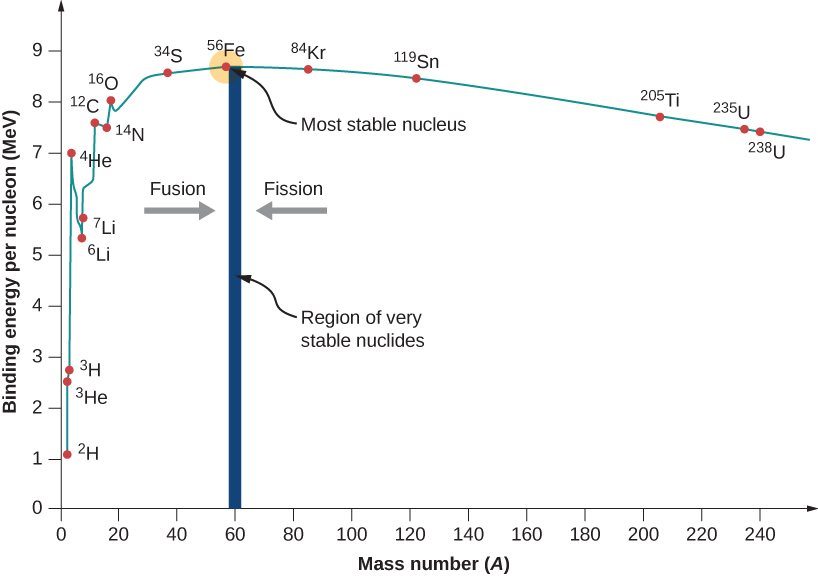
\includegraphics[width=8cm]{Binding_Energy.jpg}\\
In \textbf{nuclear fission} the binding energy per nucleon increases as a large unstable nucleus splits into two more stable fragments.\\
\\
In \textbf{nuclear fusion} the binding energy per nucleon increases, provided the nucleon number does not exceed the peak on the graph (around 50). This is why fusion can only occur on the left side of the graph as fusing iron would lose energy.\\
\\
Atoms always want to increase binding energy, fusion goes right, fission goes left.
\newpage
\section{Fission and fusion}
\subsection{Induced fission}
Fission is when a nucleus splits into two approximately equal fragments. This happens when a uranium nucleus is bombarded by neutrons and is called \textbf{induced fission}.\\
\\
Each fission event releases energy and two or three neutrons
\begin{itemize}
\item \textbf{Fission neutrons}, the neutrons released in a fission event, are capable of causing a further fission event in a \textbf{chain reaction}.
\item \textbf{Energy is released} when a fission event occurs because the fragments repel each other with sufficient charge to overcome the strong nuclear force holding them together. These nuclei and the neutrons then gain kinetic energy. The two fragment nuclei are smaller, and so have a higher binding energy than the original nucleus. The energy released is equal to the change in binding energy
\end{itemize}
\subsection{Nuclear fusion}
Fusion takes place when two nuclei combine to form a bigger nucleus. The binding energy per nucleon of the product nucleus is greater than of the initial nuclei. Energy is released equal to the binding energy.\\
\\
Fusion takes place when two nuclei combine at high speed, this is needed to overcome the electrostatic repulsion between the two nuclei so they can interact using the strong nuclear force.\\
\\
\textbf{Solar energy} is produced as a result of fusion inside the sun. The gas is at such high pressure that it turns into plasma and the nuclei have so much energy that they fuse when they collide.
\subsubsection{Fusion power}
Fusion reactors are still in prototype stage and as yet don't produce more energy than they use
\section{The thermal nuclear reactor}
\subsection{Inside a nuclear reactor}
A thermal nuclear reactor in a nuclear power station contains fuel rods spaced evenly in a steel vessel known as the \textbf{reactor core}. The reactor core also contains \textbf{control rods} and a \textbf{coolant} as well as the fuel rods and is connected by steel pipes to a \textbf{heat exchanger}. A pump is used to force the coolant through the reactor core and through the heat exchanger where it raises steam to drive turbines.\\
\\
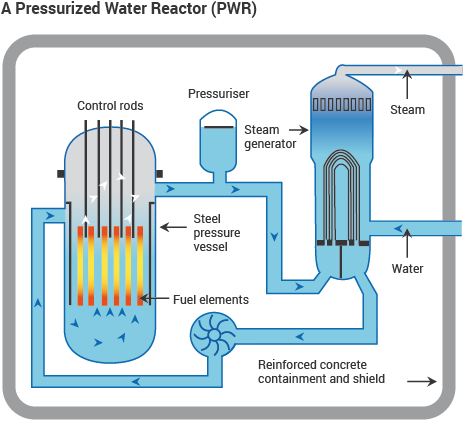
\includegraphics[width=7cm]{reactor.png}
\begin{itemize}
\item The fuel rods contain enriched uranium
\item The control rods absorb neutrons to stop chain reactions
\item The fission neutrons need to be slowed to cause further fission. The fuel rods are surrounded by a moderator so the neutrons are slowed by repeated collisions. Water acts as the moderator
\item For a chain reaction to occur the mass of the uranium must be greater than a minimum mass called the \textbf{critical mass}. This to reduce the number of escaping neutrons to allow reactions to continue
\end{itemize}
\subsection{Safety features}
A nuclear reactor needs safety features to protect workers and the environment:
\begin{itemize}
\item The reactor core is made of thick steel to withstand high pressure and temperature. This also absorbs $\beta$ and some gamma radiation and neutrons from the core
\item The core is in a building with very thick concrete walls to absorb neutrons and gamma radiation
\item Every reactor has an emergency shut-down to insert the control rods to stop fission
\item The fuel rods are inserted and removed from the reactor by remote handling devices to protect workers.
\end{itemize}
\subsection{Radioactive waste}
Radioactive waste must be stored in cooling ponds for a year as they continue to release heat due to radioactive decay.\\
This is then processed and the unused uranium is then removed and stored in sealed containers. This is then stored for centuries.\\
\\
Lower level radioactive waste is stored in drums filled with concrete.
\end{document}
